\chapter{\IfLanguageName{dutch}{Stand van zaken}{State of the art}}
\label{ch:stand-van-zaken}

% Tip: Begin elk hoofdstuk met een paragraaf inleiding die beschrijft hoe
% dit hoofdstuk past binnen het geheel van de bachelorproef. Geef in het
% bijzonder aan wat de link is met het vorige en volgende hoofdstuk.

% Pas na deze inleidende paragraaf komt de eerste sectiehoofding.

\section{Wat is autodelen?}
Autodelen bestaat ondertussen zo'n 15-tal jaar in België \autocite{ing}, autodelen is echter geen recent fenomeen. Volgens \textcite{millardball} vinden we de eerste pogingen van een vastgestelde autodeelorganisatie terug in de jaren '40 in een coöperatief samenwoon-project in het Zwitserse Zürich. Het meeste onderzoek gedaan rond autodelen geeft echter geen formele definitie van wat autodelen nu exact is \autocite{millardball}. In dit onderzoek zullen we autodelen definiëren als ``de toegang, via een abonnement of bundel, tot een vloot auto's via het zelfbedieningsprincipe, beschikbaar voor korte periodes en korte afstanden, waarvoor de gebruiker (particulier of bedrijf) een toeslag per uur en/of per afgelegde kilometer betaald`` \autocite{ing}.

\section{Wachtrijtheorie}
Een mogelijke aanpak voor het modelleren van een reservatiesysteem zoals dat van Partago is met behulp van wachtrijtheorie. In de masterthesis Dimensionering van een autodeelsysteem aan de hand van wachtrijtheorie beschrijft \textcite{van-buggenhout} hoe een reservatiesysteem gemodeleerd kan worden aan de hand van wachtrijtheorie. Verder in dit onderzoek zal er geen gebruik gemaakt worden van wachtrijtheorie, het is echter belangrijk om deze mogelijke aanpak toch kort toe te lichten. In wat volgt vatten we kort samen hoe het systeem gemodelleerd kan worden aan de hand van wachtrijtheorie.

\subsection{Wat is wachtrij theorie}
Een wachtrijmodel beschrijft een systeem waarbij klanten arriveren bij het systeem op verschillende tijdstippen, wachten tot het hun beurt is om door het systeem geserveerd te worden en tenslotte het systeem terug verlaten. Het doel van wachtrijtheorie is een balans te vinden tussen de service naar klanten toe en het aantal servers. Meer servers betekend doorgaans hogere kosten. \textcite{van-buggenhout}. Naar Partago toe kunnen we de servers vertalen naar auto's. Hoe meer auto's hoe meer klanten Partago kan serveren, maar hoe meer auto's hoe hoger de operationele kosten. 

Om het systeem correct te modelleren aan de hand van wachtrijtheorie moeten we de volgende parameters kennen:
\begin{itemize}
	\item de grootte van de populatie van klanten
	\item het type aankomstproces 
	\item de capaciteit van de wachtrij
	\item het type serviceproces
	\item het aantal beschikbare servers
\end{itemize}

\subsection{Grootte van de klantenpopulatie}
Er wordt een onderscheidt gemaakt tussen eindige en oneindige klantenpopulaties. Om gebruik te kunnen maken van de Partagoauto's moet je coöperant zijn van Partago. Het systeem kent dus ten alle tijden een bovengrens voor de klantenpopulatie en is dus eindig, namelijk het aantal coöperanten.

\subsection{Aankomstproces}
Elke Partago-coöperant heeft zijn eigen mobiliteitsbehoeften. Er wordt vanuit gegaan dat deze mobiliteitsbehoeften willekeurig en geheugenloos zijn. Geheugenloos wil zeggen dat het tijdstip van het huidige gebruik van het systeem onafhankelijk is van het vorige gebruik. Als er tijdens een bepaalde periode  $P_{1}$ een aantal reserveringen waren dan heeft dit geen invloed op hoeveel er zullen zijn in een andere periode $P_{2}$. Er wordt gesproken van willekeur omdat de reservaties niet uniform aan het systeem toekomen. Als er geweten is dat er tijdens een bepaalde periode gemiddeld 6 reservaties per uur zijn wil dit niet zeggen dat deze 6 reservaties mooi om de tien minuten plaatsvinden. Om met deze willekeur overweg te kunnen zal het aankomstproces gemodelleerd worden door middel van een statistische verdeling. Een discreet aankomstproces dat geheugenloos en willekeurig is kan gemodelleerd worden aan de hand van een Poisson-proces. Een Poisson-proces is een proces waarbij het aantal aankomsten verdeeld is volgens een Poisson-distributie terwijl de tijd tussen 2 aankomsten exponentieël verdeeld is. Een Poisson-proces wordt gekarakteriseerd volgens de aankomstsnelheid $\Lambda$ \autocite{liu}. Een belangrijke kanttekening die  hierbij gemaakt moeten worden is dat deze parameter voor het systeem van Partago wel afhankelijk is van de tijd. Zo is het weekend bijvoorbeeld drukker. Tijdens het weekend zal er dus een hogere aankomstsnelheid gemeten kunnen worden. \autocite{van-buggenhout}

\subsection{Capaciteit van de wachtrij}
Wanneer een gebruiker niet geserveerd kan worden door Partago zal deze gebruiker zijn mobiliteitsbehoeften elders moeten vervullen. Er staan dus nooit gebruikers in de wachtrij. De grootte van de wachtrij is met andere woorden nul.

\subsection{Serviceproces}
Het Partago systeem serveert een gebruiker wanneer deze gebruiker gebruik maakt van de gereserveerde auto. De service tijd wordt gedefinieerd als de tijd dat een gebruiker gebruik maakt van het systeem. De service tijden van alle gebruikers en servers zijn onafhankelijk van elkaar en worden veronderstelt exponentieel verdeelt te zijn en dus te modelleren zijn als poissonprocessen. De kans dat een gebruiker zijn gebruik van de auto beëindigt is onafhankelijk van de tijd reeds gebruik gemaakt van de auto.

\subsection{Beschikbare servers}
Het systeem bestaat uit een vast aantal auto's. Het systeem weet ook ten alle tijden welke auto's beschikbaar zijn en welke niet.

\subsection{Conclusie}
Aan de hand van wachtrijtheorie kon \textcite{van-buggenhout} een model creëren voor het Partago systeem. Dit model werd in een java-applicatie gegoten. Met behulp van deze applicatie werd de optimale vlootgrootte berekent voor de verschillende zones waar Partago actief was op het moment van schrijven van van Buggenhout's onderzoek. Als waarde voor de aankomstsnelheid voor het Poisson aankomstproces werd de aankomstsnelheid van de historisch drukste ochtend van die bepaalde zone gekozen. Uit het onderzoek werd geconcludeerd dat om het service level op 95\% te krijgen er in alle zones één auto moet bijkomen. Dit heeft echter een zeer negatief effect op de bezettingsgraad van de vloot. De impact van de verschillende parameters kan als volgt worden samengevat. 
\begin{center}
	\begin{tabular}{ | l | l | p{3cm} |}
		\hline
		Parameter & Relatie tot service level (QoS) & Impact op service level \\ \hline
		Aankomstsnelheid $A_{p}$ & $A_{p}$ $\uparrow$ = $QoS$ $\downarrow$ & hoog \\ \hline
		Aantal auto's $m$ & $m$ $\uparrow$ = $QoS$ $\uparrow$ & hoog \\ \hline
		Gemiddelde gebruikstijd $MST$ & $MST$ $\uparrow$ = $QoS$ $\downarrow$ & hoog \\ \hline
		Aantal gebruikers $S$ & $S$ $\uparrow$ = $QoS$ $\downarrow$ & laag \\ \hline
	\end{tabular}
\end{center} 
In deze bachelorproef zal echter geen gebruik gemaakt worden van wachtrijtheorie. Het onderzoek van \textcite{van-buggenhout} werd geschreven kort na de oprichting van Partago en het systeem bevond zich dus nog in een zeer vroeg stadium. Voor dit onderzoek wordt gebruik gemaakt van een grote hoeveelheid historische reservaties als input voor het uitvoeren van de simulaties. In het hoofdstuk ~\ref{ch:methodologie} wordt verder uitgelegd hoe te werk is gegaan.

\section{Constraint Satisfaction Problem}

De doelstelling van dit onderzoek is een antwoord formuleren op de vraag of het invoeren van een toewijzingsalgoritme voor de reservaties tot een hogere service level zal leiden. Een toewijzingsprobleem kan herleid worden tot een Constraint Satisfaction Problem.

\subsection{Definitie}
Het toewijzen welke reservatie zal doorgaan met welke auto kan herleidt worden tot een Constraint Satisfaction Problem in het kort een CSP. Een CSP is gedefinieerd door een set \textbf{variabelen} $X_{1}$, $X_{2},...,X_{n}$ en een set \textbf{constraints} $C_{1}, C_{2},...C_{m}$. Elke variabele $X_{i}$ heeft een niet leeg \textbf{domein} $D_{i}$ van mogelijke waarden. Elke constraint $C_{i}$ heeft betrekking tot een subset van de variabelen en specificeert de mogelijke combinaties van waarden voor deze subset. Een toestand van het probleem is gedefinieerd als een \textbf{toewijzing} van waarden aan sommige van de variabelen $X_{i} =  v_{i}, X_{j} = v_{j}$... Een toewijzing dat geen enkele van de constraints schendt is een \textbf{consistente} of legale toewijzing. Een volledige toewijzing of \textbf{oplossing} van het CSP is een toewijzing waarin alle variabelen vernoemd worden en aan alle constraints is voldaan. Soms moet een oplossing van een CSP er ook naar streven een strafscore te minimaliseren \autocite{norvig}.

\subsection{Oplossen van een CSP}
Het oplossen van een CSP is een complexe aangelegenheid. Voor het oplossen van zulke problemen worden steeds krachtigere algoritmes ontwikkeld. Een standaard algoritme kan een diepte-eerst backtracking search zijn \autocite{norvig}. Deze aanpak is relatief eenvoudig in implementatie en is ook het soort algoritme dat gebruikt wordt in de softwarebibliotheek die later in dit onderzoek gebruikt wordt.
\paragraph{Diepte-eerst zoeken}
Diepte eerst zoeken is een blinde zoekmethode. Dit wil zeggen dat ze enkel gebruik kunnen maken van de informatie verschaft in de definitie van het probleem \autocite{lievens}. Bij diepte-eerst zoeken wordt een open lijst gebruikt. Deze open lijst bestaat uit mogelijke partiële oplossingen (plannen) die nog verder geëxpandeerd moeten worden. Bij diepte-eerst zoeken wordt deze open-lijst bijgehouden in een LIFO-structuur (Last In First Out). Dit zorgt ervoor dat men steeds zo snel mogelijk zo diep mogelijk afdaalt in de zoekboom. \begin{figure}[h]
	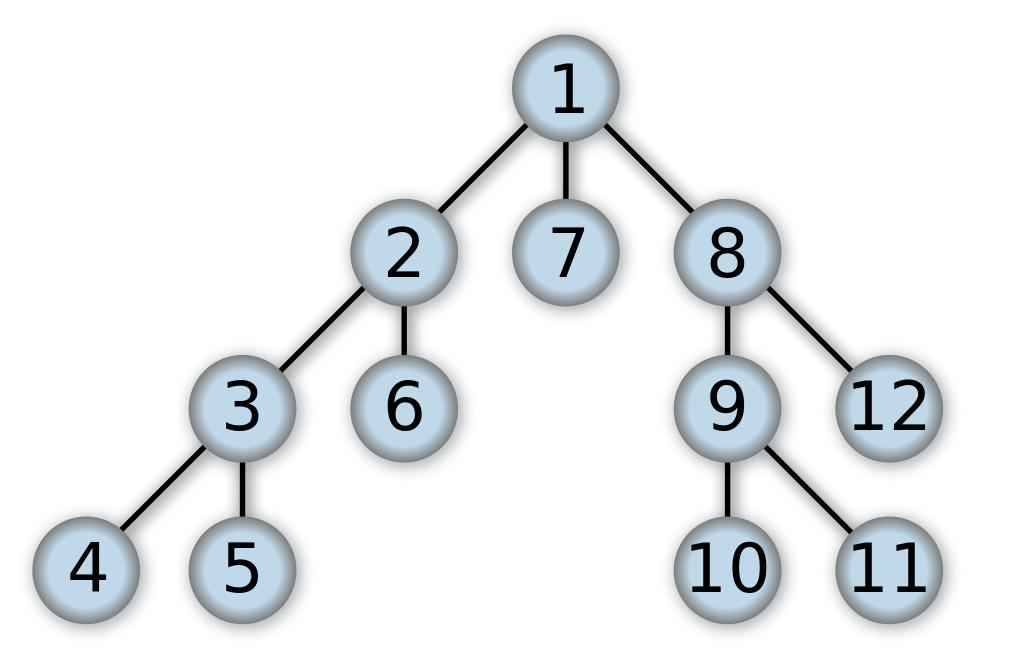
\includegraphics[width=\textwidth]{diepte-eerst.png}
	\caption{visuele voorstelling de zoekboom bij diepte-eerst zoeken}
\end{figure}
Wanneer diepte eerst een oplossing vindt is deze niet gegarandeerd een optimale oplossing. De oplossing ontdekt door diepte eerst is immers steeds de ``meest linkse`` doeltop. Wanneer het aantal verschillende mogelijke toestanden eindig is en de doeltop bevindt zich helemaal rechts onderaan de zoekboom dan worden alle toppen van de boom doorlopen door het zoekalgoritme. Diepte-eerst heeft dus in het slechtste geval een exponentiële tijdscomplexiteit van $\Theta(b_{m})$ \autocite{lievens}. $b$ is het aantal broers van een knoop in de boom (dus het aantal mogelijke domeinwaarden) en $m$ het aantal niveau's in de boom (dus het aantal variabelen).

\paragraph{Backtracking search}
Backtracking search is een algoritme dat diepte eerst te werk gaat om op zoek te gaan naar een oplossing van een CSP probleem. Het kiest waarden voor één variabele tegelijk en traceert terug in de boom wanneer er geen domeinwaarden meer mogelijk zijn om toe te wijzen aan een variabele. Eén voor een worden niet geässigneerde variabelen geprobeerd, voor elke variabele wordt dan elke domeinwaarde uitgeprobeerd \autocite{norvig}. De volgorde dat de variabelen doorlopen worden en de volgorde dat de domeinwaarden geprobeerd worden heeft een grote invloed op de uiteindelijke oplossing die het algoritme zal ``tegenkomen``. Door het wijzigen van deze volgordes op basis heuristieken  die extra informatie aan het algoritme verschaffen zal het algoritme beter presteren. Een voorbeeld van zo'n heuristiek is om de uit te proberen domeinwaarden te sorteren op de minst beperkende domeinwaarde. Met andere woorden de eerste domeinwaarde die wordt uitgeprobeerd is degene die het minst voorkomst in de constraints voor deze variabele. Jammer genoeg maakt de softwarebibliotheek die verder in dit onderzoek gebruikt wordt nog geen gebruik van deze heuristieken.

